\uuid{0MpI}
\exo7id{5409}
\titre{exo7 5409}
\auteur{rouget}
\organisation{exo7}
\datecreate{2010-07-06}
\isIndication{false}
\isCorrection{true}
\chapitre{Dérivabilité des fonctions réelles}
\sousChapitre{Théorème de Rolle et accroissements finis}
\module{Analyse}
\niveau{L1}
\difficulte{}

\contenu{
\texte{
Soit $f\in C^2([a,b],\Rr)\cap D^3(]a,b[,\Rr)$. Montrer qu'il existe $c\in]a,b[$ tel que

$$f(b)=f(a)+\frac{b-a}{2}(f'(a)+f'(b))-f^{(3)}(c).$$

Indication. Appliquer le théorème de \textsc{Rolle} à $g'$ puis $g$ où $g(x)=f(x)-f(a)-\frac{x-a}{2}(f'(x)+f'(a))-A(x-a)^3$ où $A$ est intelligemment choisi.

Que devient cette formule si on remplace $f$ par $F$ une primitive d'une fonction $f$ de classe $C^1$ sur $[a,b]$ et deux fois dérivable sur $]a,b[$~?~Interprétez géométriquement.
}
\reponse{
Pour $x\in[a,b]$, posons $g(x)=f(x)-f(a)-\frac{x-a}{2}(f'(x)+f'(a))-A(x-a)^3$ où $A$ est choisi de sorte que 
$g(b)=g(a)=0$ (c'est-à-dire $A=\frac{1}{(b-a)^3}(f(b)-f(a)-\frac{b-a}{2}(f'(b)+f'(a)))$.

$f\in C^2([a,b],\Rr)\cap D^3(]a,b[,\Rr)$ et donc $g\in C^1([a,b],\Rr)\cap D^2(]a,b[,\Rr)$. Pour $x\in[a,b]$, on a~: 
$$g'(x)=f'(x)-\frac{1}{2}(f'(x)+f'(a))-\frac{x-a}{2}f''(x)-3A(x-a)^2,$$ 

puis 

$$g''(x)=\frac{1}{2}f''(x)-\frac{1}{2}f''(x)-\frac{x-a}{2}f^{(3)}(x)-6A(x-a)=\frac{x-a}{2}(-12A-f^{(3)}(x)).$$

$g$ est continue sur $[a,b]$, dérivable sur $]a,b[$ et vérifie de plus $g(a)=g(b)$. Donc, d'après le théorème de \textsc{Rolle}, il existe $d\in]a,b[$ tel que $g'(d)=0$. De même, $g'$ est continue sur $[a,d]\subset[a,b]$, dérivable sur $]a,d[(\neq\emptyset)$ et vérifie de plus $g'(a)=g'(d)(=0)$. D'après le théorème de \textsc{Rolle}, il existe $c\in]a,d[\subset]a,b[$ tel que $g''(c)=0$ ou encore tel que $A=-\frac{1}{12}f^{(3)}(c)$ (puisque $c\neq a$).

En écrivant explicitement l'égalité $g(b)=0$, on a montré que~:

$$\exists c\in]a,b[/\;f(b)=f(a)+\frac{b-a}{2}(f'(b)+f'(a))-\frac{1}{12}f^{(3)}(c)(b-a)^3.$$

Si $f\in C^1([a,b],\Rr)\cap D^2(]a,b[,\Rr)$ et si $F$ est une primitive de $f$ sur $[a,b]$, la formule précédente s'écrit~:

$$\int_{a}^{b}f(t)\;dt=F(b)-F(a)=\frac{b-a}{2}(F'(b)+F'(a))-\frac{1}{12}F^{(3)}(c)(b-a)^3=\frac{b-a}{2}(f(b)+f(a))-\frac{1}{12}f''(c)(b-a)^3.$$

Donc, si $f\in C^1([a,b],\Rr)\cap D^2(]a,b[,\Rr)$, 

$$\exists c\in]a,b[/\;\int_{a}^{b}f(t)\;dt=\frac{b-a}{2}(f(b)+f(a))-\frac{1}{12}f''(c)(b-a)^3.$$

Interprétation géométrique.

Si $f$ est positive, $A_1=\int_{a}^{b}f(t)\;dt$ est l'aire du domaine $D=\{M(x,y)\in\Rr^2/\;a\leq x\leq b\;\mbox{et}\;0\leq y\leq f(x)\}$ et $A_2=\frac{b-a}{2}(f(b)+f(a))$ est l'aire du trapèze $\left(
\begin{array}{c}
a\\
0
\end{array}
\right)\left(
\begin{array}{c}
b\\
0
\end{array}
\right)\left(
\begin{array}{c}
b\\
f(b)
\end{array}
\right)\left(
\begin{array}{c}
a\\
f(a)
\end{array}
\right)$. Si $M_2=\mbox{sup}\{|f''(x)|,\;x\in[a,b]\}$ existe dans $\Rr$, on a~:

$$|A_1-A_2|\leq M_2\frac{(b-a)^3}{12}.$$

$$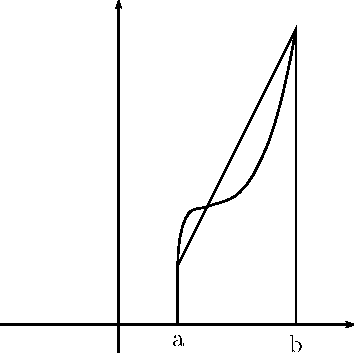
\includegraphics{../images/pdf/0MpI-1.pdf}$$
}
}
